

%% AP Physics MC Questions Archive
%%----------------------------------------


%% B-force on Moving charge
%%----------------------------------------
%\element{ap}{
%\begin{question}{b-force-charge-q01}
%    Base your answer to the following question on the diagram below which shows two large parallel conducting plates connected to a battery of emf $\varepsilon$.
%    \begin{center}
%    \begin{tikzpicture}
%        %% NOTE: TODO: draw tikz ??
%    \end{tikzpicture}
%    \end{center}
%    A magnetic field is applied in the region in between the plates such that a particle traveling to the right in this region would feel no net force.
%    What direction should this magnetic field point?
%    \begin{choices}
%        \wrongchoice{into the page}
%      \correctchoice{out of the page}
%        \wrongchoice{towards the right}
%        \wrongchoice{towards the left}
%        \wrongchoice{towards the top of the page}
%    \end{choices}
%\end{question}
%}

\element{ap}{
\begin{question}{b-force-charge-q02}
    Which combination of units can be used to express magnetic field strength?
    \begin{choices}
        \wrongchoice{kilogram meter per second per coulomb (\si{\kilo\gram\meter\per\second\per\coulomb})}
        \wrongchoice{newton meter per coulomb (\si{\newton\meter\per\coulomb})}
      \correctchoice{kilogram per second per coulomb (\si{\kilo\gram\per\second\per\coulomb})}
        \wrongchoice{newton per coulomb (\si{\newton\per\coulomb})}
        \wrongchoice{kilogram meter per coulomb (\si{\kilo\gram\meter\per\coulomb})}
    \end{choices}
\end{question}
}

\element{ap}{
\begin{question}{b-force-charge-q03}
    Which of the following explains why a magnetic field does no work on a moving charged particle?
    \begin{choices}
        \wrongchoice{The magnetic force is conservative.}
        \wrongchoice{The magnetic force depends on the speed of the particle.}
      \correctchoice{The magnetic force is always perpendicular to the direction of motion.}
        \wrongchoice{There is always an electric field that cancels the work done by the magnetic field.}
        \wrongchoice{The magnetic force depends on the direction of motion of the particle.}
    \end{choices}
\end{question}
}

\element{ap}{
\begin{question}{b-force-charge-q04}
    A particle with a charge of \SI{+3}{\micro\coulomb} and mass \SI{2e-8}{\kilo\gram} enters a \SI{0.01}{\tesla} magnetic field with a velocity of \SI{5e5}{\meter\per\second} perpendicular to the field.
    The acceleration of this particle due to the magnetic force is:
    \begin{multicols}{2}
    \begin{choices}
        \wrongchoice{\SI{1.5e5}{\meter\per\second\squared}}
        \wrongchoice{\SI{2.5e5}{\meter\per\second\squared}}
        \wrongchoice{\SI{4.5e5}{\meter\per\second\squared}}
      \correctchoice{\SI{7.5e5}{\meter\per\second\squared}}
        \wrongchoice{\SI{9.5e5}{\meter\per\second\squared}}
    \end{choices}
    \end{multicols}
\end{question}
}

\element{ap}{
\begin{question}{b-force-charge-q05}
    A particle with a mass of \SI{1.2e-5}{\kilo\gram} experiences an acceleration of \SI{2e3}{\meter\per\second\squared} as it enters a magnetic field of \SI{3}{\tesla} with a velocity of \SI{4e5}{\meter\per\second} at an angle of \ang{30} with the magnetic field.
    The magnitude of the charge on the particle is:
    \begin{multicols}{3}
    \begin{choices}
      \correctchoice{\SI{0.04}{\micro\coulomb}}
        \wrongchoice{\SI{0.4}{\micro\coulomb}}
        \wrongchoice{\SI{4}{\micro\coulomb}}
        \wrongchoice{\SI{40}{\micro\coulomb}}
        \wrongchoice{\SI{80}{\micro\coulomb}}
    \end{choices}
    \end{multicols}
\end{question}
}

\element{ap}{
\begin{question}{b-force-charge-q06}
    A particle with a charge of \SI{+2e-7}{\coulomb} and a mass of \SI{4e-4}{\kilo\gram} experiences an acceleration of \SI{3.2}{\meter\per\second\squared} due a magnetic field of \SI{8}{\tesla}.
    The velocity of the particle may be:
    \begin{choices}
        \wrongchoice{\SI{400}{\meter\per\second} perpendicular to the magnetic field.}
        \wrongchoice{\SI{400}{\meter\per\second} at an angle of 30o to the magnetic field.}
        \wrongchoice{\SI{800}{\meter\per\second} parallel to the magnetic field.}
        \wrongchoice{\SI{800}{\meter\per\second} at an angle of 30o to the magnetic field.}
      \correctchoice{\SI{800}{\meter\per\second} perpendicular to the magnetic field.}
    \end{choices}
\end{question}
}

\element{ap}{
\begin{question}{b-force-charge-q07}
    In the figure below,
    \begin{center}
    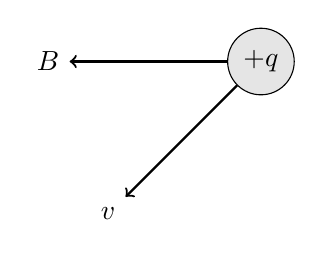
\begin{tikzpicture}
        \node[draw,circle,minimum size=0.75cm,fill=white!90!black] (A) at (0,0) {$+q$};
        \draw[thick,->] (A.west) -- ++(180:2) node[anchor=east] {$B$};
        \draw[thick,->] (A.south west) -- ++(225:2) node[anchor=north east] {$v$};
    \end{tikzpicture}
    \end{center}
        what is the direction of the particle's velocity?
    \begin{choices}
        \wrongchoice{To the left}
        \wrongchoice{To the right}
        \wrongchoice{Upward in the plane of the page}
        \wrongchoice{Out of the page}
      \correctchoice{Into the page}
    \end{choices}
\end{question}
}

\element{ap}{
\begin{question}{b-force-charge-q08}
    In the figure below,
    \begin{center}
    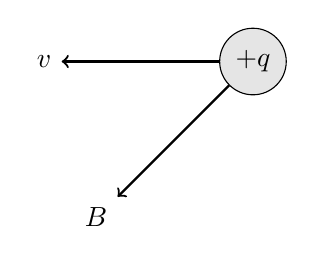
\begin{tikzpicture}
        \node[draw,circle,minimum size=0.75cm,fill=white!90!black] (A) at (0,0) {$+q$};
        \draw[thick,->] (A.west) -- ++(180:2) node[anchor=east] {$v$};
        \draw[thick,->] (A.south west) -- ++(225:2) node[anchor=north east] {$B$};
    \end{tikzpicture}
    \end{center}
        what is the direction of the magnetic force vector?
    \begin{choices}
        \wrongchoice{To the left}
        \wrongchoice{To the right}
        \wrongchoice{Upward in the plane of the page}
        \wrongchoice{Out of the page}
      \correctchoice{Into the page}
    \end{choices}
\end{question}
}

\element{ap}{
\begin{question}{b-force-charge-q09}
    In the figure below,
    \begin{center}
    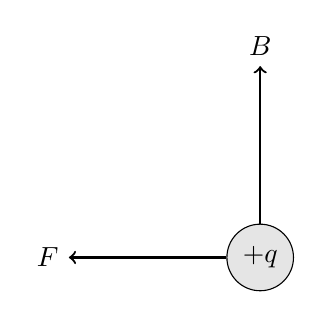
\begin{tikzpicture}
        \node[draw,circle,minimum size=0.75cm,fill=white!90!black] (A) at (0,0) {$+q$};
        \draw[thick,->] (A.north) -- ++(90:2) node[anchor=south] {$B$};
        \draw[thick,->] (A.west) -- ++(180:2) node[anchor=east] {$F$};
    \end{tikzpicture}
    \end{center}
        what is the direction of the magnetic force vector?
    \begin{choices}
        \wrongchoice{To the left}
        \wrongchoice{To the right}
        \wrongchoice{Upward in the plane of the page}
      \correctchoice{Out of the page}
        \wrongchoice{Into the page}
    \end{choices}
\end{question}
}

\element{ap}{
\begin{question}{b-force-charge-q10}
    A positron executes uniform circular motion due to the influence of a magnetic force within a uniform magnetic field $B$.
    If the positron's charge is $q$, and the linear momentum of the positron is $p$,
        find an expression for the radius of the positron's path.
    \begin{multicols}{3}
    \begin{choices}
      \correctchoice{$\dfrac{p}{qB}$}
        \wrongchoice{$\dfrac{p^2}{qB}$}
        \wrongchoice{$\dfrac{2p}{qB}$}
        \wrongchoice{$\dfrac{qB}{p}$}
        \wrongchoice{$\dfrac{qB}{p^2}$}
    \end{choices}
    \end{multicols}
\end{question}
}

\element{ap}{
\begin{question}{b-force-charge-q11}
    A particle executes uniform circular motion with speed $v$ due to the influence of a magnetic force within a uniform magnetic field $B$.
    If the particle's charge is $q$,
        and the radius of the path of the particle is $r$,
        find an expression for the mass of the particle.
    \begin{multicols}{3}
    \begin{choices}
      \correctchoice{$\dfrac{rqB}{v}$}
        \wrongchoice{$\dfrac{rqB}{v^2}$}
        \wrongchoice{$rqvB$}
        \wrongchoice{$\dfrac{v}{rqB}$}
        \wrongchoice{$\dfrac{v^2}{rqB}$}
    \end{choices}
    \end{multicols}
\end{question}
}

\element{ap}{
\begin{question}{b-force-charge-q12}
    A proton traveling at \SI{1.6e7}{\meter\per\second} enters a region with a uniform magnetic field of strength \SI{4}{\tesla}.
    If the proton's initial velocity vector makes an angle of \ang{45} with the magnetic field,
        what is the speed of the proton \SI{1}{\second} after entering the magnetic field?
    \begin{multicols}{2}
    \begin{choices}
        \wrongchoice{\SI{2.4e6}{\meter\per\second}}
        \wrongchoice{\SI{3.2e6}{\meter\per\second}}
      \correctchoice{\SI{1.6e7}{\meter\per\second}}
        \wrongchoice{\SI{2.4e7}{\meter\per\second}}
        \wrongchoice{\SI{3.2e7}{\meter\per\second}}
    \end{choices}
    \end{multicols}
\end{question}
}

\element{ap}{
\begin{question}{b-force-charge-q13}
    %% Base your answers to questions 13 and 14 on the following.
    Traveling at an initial speed of \SI{1.2e6}{\meter\per\second},
        a particle (mass = \SI{6e-10}{\kilo\gram}, charge = \SI{1.0e-10}{\coulomb})
        enters a region of uniform magnetic field with a strength of \SI{300}{\tesla} at an angle of \ang{30} to the field.
    %% start question
    What is the magnitude of the acceleration of the particle?
    \begin{multicols}{2}
    \begin{choices}
        \wrongchoice{\SI{9.0e-3}{\meter\per\second\squared}}
        \wrongchoice{\SI{1.8e-2}{\meter\per\second\squared}}
      \correctchoice{\SI{3.0e7}{\meter\per\second\squared}}
        \wrongchoice{\SI{7.2e7}{\meter\per\second\squared}}
        \wrongchoice{\SI{3.0e17}{\meter\per\second\squared}}
    \end{choices}
    \end{multicols}
\end{question}
}

\element{ap}{
\begin{question}{b-force-charge-q14}
    %% Base your answers to questions 13 and 14 on the following.
    Traveling at an initial speed of \SI{1.2e6}{\meter\per\second},
        a particle (mass = \SI{6e-10}{\kilo\gram}, charge = \SI{1.0e-10}{\coulomb})
        enters a region of uniform magnetic field with a strength of \SI{300}{\tesla} at an angle of \ang{30} to the field.
    %% start question
    What is the speed of the particle after \SI{1}{\second}?
    \begin{multicols}{2}
    \begin{choices}
        \wrongchoice{\SI{6.0e5}{\meter\per\second}}
      \correctchoice{\SI{1.2e6}{\meter\per\second}}
        \wrongchoice{\SI{3.0e6}{\meter\per\second}}
        \wrongchoice{\SI{4.2e6}{\meter\per\second}}
        \wrongchoice{\SI{5.4e6}{\meter\per\second}}
    \end{choices}
    \end{multicols}
\end{question}
}

\element{ap}{
\begin{question}{b-force-charge-q15}
    An electron enters a uniform magnetic field $B$ pointing out of the page while traveling at a velocity $v$ to the right,
        perpendicular to the field.
    Which of the following best describes the path of the electron within the uniform magnetic field $B$?
    \begin{choices}
        \wrongchoice{The path of the particle is unchanged, but it speeds up.}
        \wrongchoice{The path of the particle is unchanged, but it slows down.}
        \wrongchoice{A clockwise circular path.}
      \correctchoice{A counterclockwise circular path.}
        \wrongchoice{The electron will come to rest.}
    \end{choices}
\end{question}
}

\element{ap}{
\begin{question}{b-force-charge-q16}
    A particle with charge $+q$ is traveling through a uniform magnetic field $B$ that points out of the page in the direction indicated by the arrow in the plane of the page.
    \begin{center}
    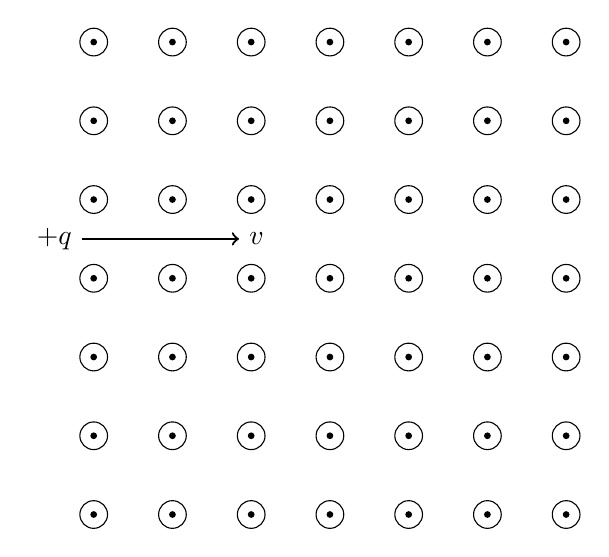
\begin{tikzpicture}
        %% magnetic field
        \foreach \x in {-3,-2,...,2,3}
            \foreach \y in {-3,-2,...,2,3} {
                \draw (\x,\y) circle (5pt);
                \draw[fill] (\x,\y) circle (1pt);
            }
        %% Velocity
        \node[anchor=center] (A) at (-3.5,0.5) {$+q$};
        \draw[thick,->] (A.east) -- ++(0:2cm) node[anchor=west] {$v$};
    \end{tikzpicture}
    \end{center}
    In what direction is the force on the particle?
    \begin{choices}
      \correctchoice{towards the bottom of the page}
        \wrongchoice{towards the top of the page}
        \wrongchoice{up out of the page}
        \wrongchoice{down into the page}
        \wrongchoice{towards the left of the page}
    \end{choices}
\end{question}
}

\element{ap}{
\begin{questionmult}{b-force-charge-q17}
    In order for a magnetic field to exert a force on an object,
        which of the follow can be true?
    \begin{choices}
      \correctchoice{The object is charged.}
        \wrongchoice{The object is moving parallel to the field.}
      \correctchoice{The object is moving perpendicular to the field.}
        %\wrongchoice{I only}
        %\wrongchoice{II only}
        %\wrongchoice{III only}
        %\wrongchoice{I and II only}
        %\correctchoice{I and III only}
    \end{choices}
\end{questionmult}
}

\element{ap}{
\begin{question}{b-force-charge-q18}
    A magnetic field exerts a non-zero force on a particle.
    Which of the following must be true?
    \begin{choices}
        \wrongchoice{The particle is negatively charged.}
        \wrongchoice{The particle is stationary.}
        \wrongchoice{The direction of the force is perpendicular to the magnetic field but parallel to the motion of the particle.}
        \wrongchoice{The direction of the force is parallel to the magnetic field but perpendicular to the motion of the particle.}
      \correctchoice{The direction of the force is perpendicular to both the velocity of the particle and the magnetic field.}
    \end{choices}
\end{question}
}

\element{ap}{
\begin{question}{b-force-charge-q19}
    Base your answer to the following question on the diagram below.
    \begin{center}
    \begin{tikzpicture}
        \draw (-0.3,2) arc (180:0:0.3cm and 0.1cm) -- (0.3,-2) arc (360:180:0.3cm and 0.1cm) --cycle;
        \draw (-0.3,2) arc (180:360:0.3cm and 0.1cm);
        %% elelctron
        \node[anchor=center] (E) at (0,-1) {$e^-$};
        \draw[thick,->]  (E.north) -- ++(90:2);
        %% point P
        \draw[fill] (3,0) circle (1.5pt) node[anchor=west] {$P$};
    \end{tikzpicture}
    \end{center}
    If a positively charged particle is placed at point $P$,
        the force due to the magnetic field:
    \begin{choices}
        \wrongchoice{increases with increasing charge}
        \wrongchoice{is opposite the direction of the magnetic field}
      \correctchoice{is zero}
        \wrongchoice{is in the direction of the magnetic field}
        \wrongchoice{causes the particle to accelerate to the right}
    \end{choices}
\end{question}
}


\endinput


